\documentclass[tikz,border=2pt]{standalone}
\usepackage{amsmath}
\usepackage{xcolor}
\definecolor{bg}{HTML}{171D2B}
\definecolor{aksen}{HTML}{F7B538}
\definecolor{biru}{HTML}{7DD3FC}
\pagecolor{bg}
\color{white}
\begin{document}
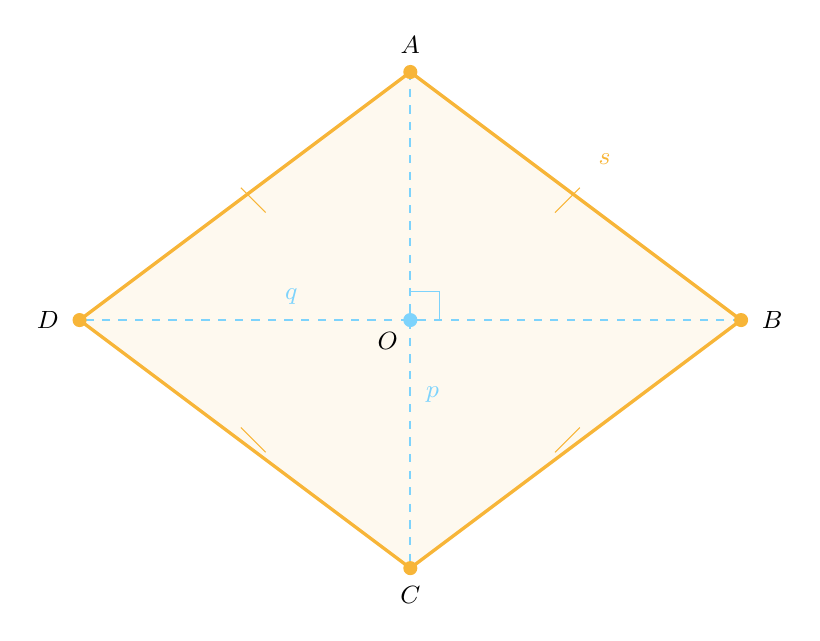
\begin{tikzpicture}[scale=1.05,>=stealth,
  titik/.style={circle,fill=aksen,inner sep=1.8pt}]

  % Belah ketupat: A(0,3), B(4,0), C(0,-3), D(-4,0)
  \coordinate (A) at (0,3);
  \coordinate (B) at (4,0);
  \coordinate (C) at (0,-3);
  \coordinate (D) at (-4,0);
  \coordinate (O) at (0,0);

  % Isi transparan
  \fill[aksen,opacity=0.08] (A) -- (B) -- (C) -- (D) -- cycle;

  % Sisi
  \draw[very thick,aksen] (A) -- (B) -- (C) -- (D) -- cycle;

  % Diagonal
  \draw[thick,biru,dashed] (A) -- (C) node[pos=0.65,right=2pt,font=\small] {$p$};
  \draw[thick,biru,dashed] (B) -- (D) node[pos=0.68,above=2pt,font=\small] {$q$};

  % Tanda sisi sama panjang (satu tick tiap sisi)
  \draw[aksen] (1.9,1.45) +(-0.15,-0.15) -- +(0.15,0.15);
  \draw[aksen] (-1.9,1.45) +(0.15,-0.15) -- +(-0.15,0.15);
  \draw[aksen] (1.9,-1.45) +(0.15,0.15) -- +(-0.15,-0.15);
  \draw[aksen] (-1.9,-1.45) +(-0.15,0.15) -- +(0.15,-0.15);

  % Sudut siku di O
  \draw[biru] (0,0.35) -- (0.35,0.35) -- (0.35,0);

  % Siku di titik A (garis AB tegak lurus AC? tidak -- siku antara sisi dan diagonal? skip)

  % Titik dan label
  \node[titik] at (A) {}; \node[above=3pt] at (A) {\small $A$};
  \node[titik] at (B) {}; \node[right=4pt] at (B) {\small $B$};
  \node[titik] at (C) {}; \node[below=3pt] at (C) {\small $C$};
  \node[titik] at (D) {}; \node[left=4pt] at (D) {\small $D$};
  \node[titik,fill=biru] at (O) {}; \node[below left=1pt] at (O) {\small $O$};

  % Panjang sisi
  \node[font=\small\color{aksen}] at (2.35,1.95) {$s$};
\end{tikzpicture}
\end{document}
